

\section{\DSU{} DSU Implementation}
\label{sec:vm}

This section describes how we support DSU in \DSU{} by extending
common virtual machine services.  \DSU{} is built on the
\JikesRVM{},
a high-performance Java-in-Java Research VM~\cite{AAB+:99,VMperf:webpage}.
\DSU{} integrates and extends the \JikesRVM{}'s dynamic classloader,
JIT compiler, thread scheduler, copying garbage collector (GC), and
support for return barriers and on-stack replacement to implement DSU\@.  
%MWH: we mention this below.  I don't think this is such a technical
%advance that we need to call it out here.  If you want to put it
%back, add the citation, I think.
% We also added a
% generic return-barrier mechanism to \JikesRVM\@.

%MWH: detail that won't make much sense here.
% Both \emph{class updates} and \emph{method body updates}
% require VM
% % \emph{method body updates} (see Section~\ref{sec:updates}), require VM
% classloading, JIT compilation, and thread scheduling support.
% \emph{Class updates} may additionally require GC and OSR support.

After the user prepares and tests a program's modifications, the
update process in \DSU{} proceeds in five steps. 
(1)~Our UPT generates an update specification.  
(2)~The user signals \DSU{}.  (3)~\DSU{} stops running threads at a DSU safe point. (4)~It loads the
updated classes, the transformer functions,
and installs the modified methods and classes. (5)~\DSU{} then
applies object and class transformers following a modified GC\@.

\subsection{Preparing the update}
\label{sec:prep}

To determine the changed and transitively-affected classes for a given
release, we wrote a simple \acf{UPT}\footnote{\ac{UPT} is built using
jclasslib: \url{http://www.ej-technologies.com/products/jclasslib}.} that examines differences between
the old and new classes provided by the user.
\ac{UPT} groups changes into three categories, and lists them in the
update specification file:

\begin{description}
\item[Class updates:] These updates change the class signature by
  add\-ing, removing, or changing the types of fields and methods.
\item[Method body updates:] These updates change only the internal
implementation of a method. 
\item[Indirect method updates:] These are methods whose bytecode is
  unchanged, but the VM recompiles them because they
  refer to fields and methods of updated classes.   The compiled
  code uses hard-coded field offsets, and the update may change these offsets.
\end{description}

\noindent  \ac{UPT} generates default object and class transformer
functions for all class updates, which the programmer may optionally
modify.  After compiling the transformers with our custom JastAdd compiler
(described in Section~\ref{subsec:transformers}), the user initiates the update by signaling the
\DSU{} VM and providing the new version of the application, the 
update specification file, and the transformers class file.


\subsection{DSU safe points}
\label{sec:safe}

\DSU{} requires the running system to reach a \emph{DSU safe point}
before it applies updates.  DSU safe points occur at \emph{VM safe
  points} but further restrict the methods on the threads' stacks.
These restrictions provide sensible update semantics: no
code from the new version executes before the update completes, and no
code from the old version executes afterward.  As mentioned in
Section~\ref{sec:overview}, we divide restricted methods into three
categories: (1) methods whose bytecode has changed, due to a class
update or a method body update; (2) methods whose bytecode has not
changed but that access an updated class; and (3) methods the user
blacklists.

This subsection next discusses why these restrictions improve the safety
and semantics of updates, and then describes the actions \DSU{}
takes to reach a DSU safe point.


\paragraph{Semantics of DSU safe points.}

Our choice of restricted methods is similar to other DSU
systems~\cite{ritzau00dynamic,Mala00a,altekar05opus,eaddy05enc,JVMhotswap,VSEnC,chen:icse07,K42reconfig}.
To understand why category~(1) methods are restricted,
consider the update from Figure~\ref{fig:email-example}.  Assume the
thread is stopped at the beginning of the
{\tt ConfigurationManager.loadUser} method. If the update takes
effect at this point, the new implementation of
{\tt User.setForward\-ed\-Ad\-dresses} will take an object of type
{\tt EmailAddress[]} as its argument.  However, if the old version
of {\tt loadUser} were to resume, it would still call
{\tt set\-Forwarded\-Addresses} with an array of {\tt String}s,
resulting in a type error.

Preventing an update until changed methods are no longer
on the stack  
ensures type safety because when the new version of the program resumes it
will be self consistent.  If a 
programmer changes the type signature of a method {\tt m}, for the program to
compile properly, the programmer must also change any methods that
call {\tt m}.  
In our example, the fact that {\tt setForwardedAddresses}
changed type necessitated changing the function {\tt loadUser} to
call it with the new type.  With this safety condition, there is no
possibility that the signature of method
{\tt m} could change and some old caller could call it---the update must also
include all updated callers of {\tt m}.

Category~(2) methods are more subtle.  Suppose some method \texttt{getStatus}
calls method \texttt{getForwardedAddresses} from our example, but
\texttt{getStatus} 
source code and bytecode has not changed from versions 1.3.1 to 1.3.2.
Nevertheless, \texttt{getStatus}'s \emph{machine code}, produced by the
JIT compiler, may need to be recompiled.  For example, if the new
compiled version of {\tt getForwarded\-Addresses} is at a different offset 
than before, then the VM must recompile
%MWH: killed extra text to avoid bad line break
\texttt{getStatus} to correctly refer to the new
offset.  An update may also change field offsets in modified classes,
which requires recompiling any class that accesses
them as well.  
Ginseng~\cite{neamtiu06dsu} and POLUS~\cite{chen:icse07}, two
DSU systems for C, likewise consider functions as changed if their
source code is the same but they
access data types whose (compiled) representation is different.
Note that the VM would not need to restrict category~(2) methods if it used an
interpreter that looked up offsets at each access.
%MWH: static offsets is redundant---these are fields, too.

%   The compiler records its inlining
% decisions and \DSU{} restricts these methods as well.
% , when an update is available,
% computes a transitive closure of all methods that have inlined methods
% appearing in the changed set.
% \DSU{} adds these additional methods to the set of restricted methods
% used to determine a safe point.
% \suriya{\DSU{} does not compute this transitive closure. It only checks for
% this information when it encounters an opt compiled method on stack.}
% \ksm{I guess we care--is the above correct enough?}


% enough---we must also restrict those methods updated indirectly, 
% because these methods
% depend on the particular field and method offsets of the classes to
% which they refer, and 
% must be recompiled.  

Even if a method has not changed, a user may need to manually blacklist it.  
For example, suppose a method \texttt{handle} calls
methods \texttt{process} and \texttt{cleanup}, and the method
\texttt{cleanup} initializes a field that it uses.  Now suppose we
update this program to move the initialization statement into
\texttt{process}, because \texttt{process} needs to use the
field as well.  In both versions, the field is properly
initialized when the program runs from scratch.  However, suppose that
\DSU{}  applies the update and the thread running \texttt{handle}
yields in between the calls to \texttt{process} and \texttt{cleanup}.
In this case, \texttt{handle}'s bytecode has not been changed
(\texttt{process} and \texttt{cleanup} are method body changes, not
class updates), so we
could go ahead with the update.  But if we did, then the program would
have called the old \texttt{process} method, which did not perform any
initialization, and then would call the new
\texttt{cleanup} method, which performs no initialization either,
since it the new version \texttt{process} does it, leading to incorrect semantics.  % As
% a result, the program will fail with a null pointer exception.
To avoid
such \emph{version consistency}
problems~\cite{neamtiu08context} the programmer can include
\texttt{handle} in the restricted set.  Our benchmarks did not require 
manual restrictions.

%MWH: moved here from prior to previous para before. I don't
%understand why it was there.  I don't understand why it was "on the
%other hand" either.  I tried to explain a bit more why we restricted
%the parent inlined method.
Finally, note that when the VM JIT compiler uses inlining we may need
to increase the 
number of restricted methods to include those into which restricted
methods are inlined.  In particular, if a
category~(1),~(2), or~(3) method {\tt m} is inlined into method {\tt
  n}, we should also restrict {\tt n} (and recompile it, after the
update) to prevent the old {\tt m} from running after the update.
\JikesRVM{} 
initially compiles a method with its \emph{base}-compiler, which
generates machine code but does not apply sophisticated
optimizations. Based on run-time profiling information, the VM may
recompile the same method later using its \emph{opt}-compiler, which performs
standard optimizations, including inlining.
It performs inlining of small, frequently used methods; cost-based
inlining for larger methods; and may inline multiple levels down a hot call chain.  
% As a consequence, \DSU{} restricts methods into which the
% \emph{opt} compiler has inlined restricted methods. 
As a consequence, \DSU{} restricts inlined callers of restricted methods.

\paragraph{Reaching a DSU safe point.}
To safely perform VM services such as thread scheduling, garbage
collection, and JIT compilation, \JikesRVM{} (like most production
VMs) inserts yield points on all method entries, method exits, and
loop back edges.  If the VM wants to perform a garbage collection or
schedule a higher priority thread, it sets a yield flag, and the
threads stop at the next VM safe point.  
\DSU{} piggybacks on this functionality.  When \DSU{} is informed that an
update is available, it sets the yield flag.  Once application threads
on all processors have reached VM safe points, \DSU{} checks the
paused threads' stacks.  If no stack refers to a restricted
method, \DSU{} applies the update.  

If any thread is running a restricted
method, \DSU{} defers the update and installs a \emph{return
  barrier}~\cite{return-barrier} on the topmost restricted method of each thread.  
A generic return barrier replaces the regular method return branch
back to the next instruction in the calling method with a branch to
\emph{bridge code}, which performs some special action and then
executes the return branch.  We added this generic return barrier
functionality to \JikesRVM\@, but this technology is standard in other
VMs.  Our bridge code restarts the update process.
Therefore, when a restricted method returns,
the thread will block and \DSU{} will restart the update process, which will
either reach a DSU safe 
point, or the VM will insert more return barriers.  If \DSU{} does not reach a safe
point within 15 seconds, it aborts the update (the
length of timeout is arbitrary, and can be configured by the user).
However, it turns out we can sometimes proceed with an update despite
category~(2) methods on-stack, as described next.

\paragraph{Lifting category (2) restrictions.} 
\DSU{} reduces the number of restricted methods in category~(2) by leveraging
VM support for on-stack replacement (OSR).  \JikesRVM{} normally uses OSR to
replace a \emph{base}-compiled version of an active method with an
optimized version.  We observe that for category~(2) restricted
methods, the situation is much the same: an unchanged, on-stack method
requires recompilation, in our case to fix any changed offsets. If the stack only contains category~(2) methods, \DSU{} first performs OSR, and then starts the update.
As of this writing, we only support OSR for \emph{base}-compiled category~(2) methods,
which do not contain any inlined calls, though we plan to support OSR
on \emph{opt}-compiled methods as well.

\JikesRVM{}'s standard OSR functionality works as follows.
After reaching a yield point, OSR recompiles the 
topmost method on a thread's stack.  % OSR takes effect when the thread running the
% to-be-recompiled method reaches a yield point.  Having compiled an
% optimized version, 
The VM then modifies the thread's current PC to switch to
the equivalent location in the new implementation, and adjusts the
stack to reflect the recompiled version.  \JikesRVM{}
examines the active stack frame and extracts the values of local
variables. It generates a special prologue to the recompiled method
that sets up a stack frame with these extracted values. The last instruction
in this prologue jumps to the new PC location. The VM then overwrites the
return address of the yield point function to jump to the prologue.

We  extend \JikesRVM's OSR facilities to support multiple stack
activation records, and multiple stack frames on the same stack. This later addition makes it more likely to reach a DSU safe point when a string of category~(2) methods precede a changed
method on the stack.
% \suriya{the next sentence can go. the method we OSR is not the void method.
% the void method is the yieldpoint method. just a piece of technical detail}
% we also extended \JikesRVM{} to enable OSR on methods that
% return values, as the standard version only handles \texttt{void}
% methods.  
Given this support, \DSU{} ignores \emph{base}-compiled category~(2) methods
when testing for a safe point.  If any \emph{base}-compiled category~(2)
methods are on stack at an otherwise DSU-safe point, \DSU{} uses OSR
to replace them.  The exact timing of OSR for DSU requires the VM to
first load modified classes, as explained next.


% mwh: from suriya's e-mail, in case we want to put some of this
% information into the text above.
% 1. how we use OSR for DSU.
%   we discover which methods should OSRed. if the vm is in a safe state for
%   DSU, we proceed with the update and OSR the chosen methods. this
%   involves using the old bytecode stream and extracting the state of the
%   stack frame, and "specially" recompiling the new bytecode stream that
%   will restore the stack frame and resume execution at the right point.
%   the main thing we have to do is set up data structures appropriately so
%   that we deal with the right class, method and bytecode data structures.
% 2. how jikesrvm does DSU.
%   jikesrvm looks at a stack frame and knows what the state of local
%   variables in the frame is. from the return address the vm also knows the
%   bytecode to resume execution at. it compiles a version of the method
%   with a special prologue (expressed in bytecode). this prologue correctly
%   sets up local variables. it also correctly gets the return value (which
%   would not have been available when the state extractor looked at the
%   stack) from the callee. the last instruction of the special prologue
%   jumps to the right execution point within the method.

\subsection{Installing modified classes}
\label{sec:loading}

Once the program reaches a safe point, \DSU{} begins the update by
loading and installing the changed classes, and updating relevant
metadata in the existing versions.

\begin{figure*}[t]
% \begin{center}
% \begin{tabular}{c|c|c}
% \scalebox{.7}{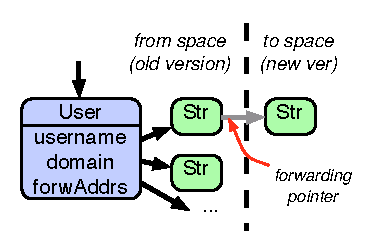
\includegraphics{gcupdate-simple1}} &
% \scalebox{.7}{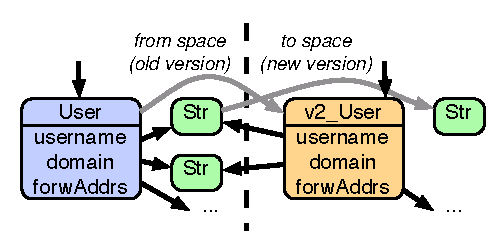
\includegraphics{gcupdate-simple2}} &
% \scalebox{.7}{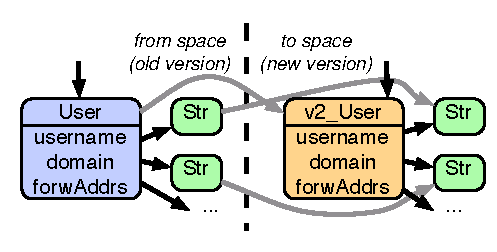
\includegraphics{gcupdate-simple3}} \\
% (i) before running transformer &
% (ii) after running transformer &
% (iii) gc+update complete \\
% \multicolumn{3}{c}{}\\
% \end{tabular}
% 
% (a) running the default transformer during the gc
% \end{center}
% \hrule
\begin{center}
\scalebox{.75}{\includegraphics{images/gcupdate}}
% 
% (b) running transformers following gc
\end{center}
\caption{Running object transformers following GC}
% \caption{copying and transforming updated objects with the gc}
\label{fig:gc-example}
\end{figure*}

\JikesRVM{} represents  classes with several internal data structures.
Each class has an \VMClass{} meta-object that describes
the class.  It points to other meta-objects that describe the class's
method and field types and offsets in an object instance.  
The compiler and garbage collector query this metadata.  Often the
compiler can statically determine the type of the object reference. In
this case, it queries the meta-object and hard-codes constant offsets
into the machine code to generate efficient field and method access
code.
The garbage collector uses meta-objects to identify object reference fields and
trace the referent objects.
\VMClass{} also stores a \emph{type information block} (TIB) for each
class, which maps a method's offset to its actual implementation.
\JikesRVM{} always compiles a method directly to machine
code when the method is first invoked.  Each object instance
contains a pointer to its TIB, to support dynamic dispatch.  When the
program invokes a method on an object, the generated code
indexes the object's TIB at the correct offset and jumps to the
machine code.

For a class with only method body updates, all of the class's metadata
is the same in both the old and new versions.  Therefore, \DSU{} invalidates the TIB entries for each replaced method, 
reads in the new method body implementations, and modifies the
existing class metadata to refer to the replacement methods' bytecode.  The JIT
will compile the updated method when the program next invokes it, after the
update.

For a class update, the class's number, type, and order of fields or
methods may have changed, which in turn impacts the class's metadata,
including its TIB\@.  \DSU{} modifies existing class metadata as
follows.  First, it changes the old class's metadata to use a
modified class name, e.g., metadata for class \texttt{User} is renamed
to \texttt{v131\_User} in our example update from
Figure~\ref{fig:email-example} and~\ref{fig:example-xform}.  Next, it
installs the new \VMClass{} and corresponding metadata
for the new version. Then the VM updates several \JikesRVM{} data
structures (e.g., the Java Table of Contents for
{\tt static} methods and fields) to indicate that the newly-loaded
class is now the up-to-date version.  Note that all TIB entries for
the newly-installed class are invalid, so all methods in the class
will be compiled on demand.  \DSU{}  invalidates the
TIB entries and other data structures for the old class so that they
can be garbage-collected.  

Once method and class updates are installed, if category~(2) methods are
active, the VM initiates OSR for these methods. 

Invalidating changed methods will impose overhead on the execution
just following the update when these methods are first
\emph{base}-compiled and then when they are progressively optimized at
higher levels, if they execute frequently.  We could reduce this
overhead somewhat by optimizing new versions directly to their prior
level of optimization.  Updates to method bodies however invalidate
execution profiles and  without branch and call frequencies, code quality
would degrade. Thus, we believe it is better to let the adaptive
compiler work as it was intended.  In any case, since dynamic updates
are relatively rare events, any added overhead due to recompilation
will be short-lived.

\subsection{Applying Transformers}
\label{sec:xformers}

We modify the \JikesRVM{}
semi-space copying collector \cite{BCM:04} to 
update changed objects as part of a collection. 
The collector transforms old objects of an updated classes to conform
to their new class signature and point to their new TIB.
A semi-space copying collector normally works by traversing the
pointer graph in the old heap (called \emph{from-space}) starting at
the \emph{roots} and performing a transitive closure over the object
graph, copying all objects it encounters to a new heap (called
\emph{to-space}).  The roots include statics, stack-allocated local variables, and references in registers.  The compiler generates a
\emph{stack map} at every VM safe point (a superset of DSU safe
points).  The stack map enumerates all register and local variables on
the stack that reference heap objects.  When the collector first
encounters an object, it copies it to to-space and then overwrites
its header with a forwarding pointer to the new copy.  If the
collector encounters a forwarded object later via another reference,
it uses the forwarding pointer to redirect the reference to the new
object.

Our modified collector works in much the same way, but differs in how
it handles objects whose class signature has changed.  In this case,
it allocates a copy of the old object \emph{and} a new object of the new
class, which may have a different size compared to the old one. The collector
initializes the new object to point to the TIB of the new type, and
installs the forwarding pointer in from-space to this new version. Next,
the collector stores a pair of pointers in its \emph{update log}, one
to the copy of the old object and one to the 
new object.  The collector continues scanning the old copy.

After the collection completes, \DSU{} first executes transformers for all
classes and then for all objects. 
%MWH: either order does not work equally well; both are wrong, really,
%but the current order is less likely to be wrong. See long e-mail
%exchange with %Suriya a while back.  We don't really handle this case
%correctly right now, so better to say little.
\DSU{} goes
through the update log and invokes the object transformer, passing
the old and new object pair as arguments.  Once it processes all
pairs, the log is deleted, making the  duplicate
old versions unreachable.  
Since they are unreachable, the next garbage collection will naturally
reclaim them.  If we put them in a special space, we could reclaim
them immediately.%   \mwh{Say why class transformers come last, and
%   ordering issues, generally?}

\paragraph{Example.}
Figure~\ref{fig:gc-example} illustrates a part of the heap at the end
of the GC phase while applying the update from
Figure~\ref{fig:example-xform} (forwarding pointers not shown).  On the left is a depiction of part of the heap prior
to the update.  It shows a {\tt User} object whose fields point to
various other elided objects.  After the copying phase, all of the old
reachable objects are duplicated in to-space.  The
transformation log points to the new version of {\tt User} (which
is initially empty) and the duplicate of the old version, both of
which are in to-space.  The transformer function can safely copy
fields of the {\tt from} object. The figure shows that after
running the transformer function, the new version of the object points
to the same {\tt username} field as before, and it points to a new
array which points to new {\tt EmailAddress} objects. The
{\tt EmailAddress} constructor called within the transformer function initialized these objects by
referring to the old e-mail 
{\tt String} values and assigning fields to point to substrings of
the given {\tt String}.

In our example, the {\tt jvolveObject} function only copies the
contents of the old {\tt User} object's fields.  More generally,
our update model allows old object fields to be dereferenced in
transformer functions so long as the fields point to transformed
objects.  If some object $o$ is dereferenced while running $p$'s
transformer method, but $o$ has not yet been transformed, we must
find $o$ and pass it and its uninitialized new version to the
{\tt jvolveObject} method to initialize
it.  Since $p$ points to the new version of $o$, we could scan the
remainder of the update log to find the old version.  To avoid
this cost, we instead cache a pointer to the old
version in the new version during the collection.
We take care that {\tt jvolveObject} functions
invoked recursively in this manner do not loop infinitely,
which would constitute one or more ill-defined transformer
functions. We detect cycles with a simple check, and abort the update.
In our current implementation, the programmer uses a
special VM function to force a field's referenced object to be
transformed.  We should be able to handle this case
automatically, through a read barrier or a simple analysis of the {\tt
  jvolveObject} bytecode.  
%FIXME

% \suriya{Reviewer 3 asks us
% to elaborate limitations of transformation functions} \suriya{Reviewer 2
% wants to talk about the problematic situation as well in a more concrete
% way. KSM: we do both as much as we understand it in related work and I point to it in the discussion below.}

% \mwh{mention what happens to deleted objects ...? fixed above }

\subsection{Discussion}
%MWH: moved this. Makes more sense in 2.3
% %MWH: leaving this here, but probably it belongs in 2.3 instead...
% In our update model, if a transformer dereferences an object reference
% which also refers to a transformed object, it refers to the new
% version.  Our experience and that of others%
% ~\cite{k42usenix,neamtiu06dsu,neamtiu09stump,upstare}
% indicate that this model expresses many updates well.  Boyapati et
% al.~\cite{boyapati03lazy} also forbid cycles, but in their model,
% transformers only reference old objects. We explain their model in
% more detail in Section~\ref{sec:related}. We leave to future work a
% detailed investigation of the semantics and expressiveness of both models.

Our implementation of object transformers uses an extra copy of all updated objects and adds
temporary memory pressure.
We  could instead copy the old versions to a special block of memory
and reclaim it when the collection completes. We could attempt to avoid
extra copies altogether by invoking object 
transformer functions during collection.  This approach is more
complicated because our transformer model requires recursively invoking the collector
from the transformer if a dereferenced field has not yet been
processed.  We also would need to use a  GC-time read barrier
to follow forwarding pointers before dereferencing an object in order
to determine whether an object has been transformed.

% In addition, to provide access to the fields 
% of changed objects in transformer functions, we can customize the
% collector to completely process the children first using a postorder
% traversal.  This traversal order would guarantee that any object
% reachable from the object transformer function is sure already initialized.
% Other programming 
% interfaces are possible, too.  For example, Boyapati et al.~\cite{boyapati03lazy}
% take advantage of encapsulation information to allow transformer code
% to access the old versions of pointed-to objects.  Our approach allows
% programs to only see the new versions of objects within transformers,
% similar to the \emph{representation consistency} invariant proposed by
% Stoyle et al.~\cite{StoyleHBSN06}.  We will let future experience
% guide our understanding of which programming interfaces are most
% useful.

% These disadvantages have not proved problematic in practice.  Very often the
% default transformer is sufficient, in which case there is no extra copying.
% The custom object transformer functions we have written are similar to the
% one in Figure~\ref{fig:example-xform}.  By and large, they copy fields
% (either base types or pointers) from the old object to the new one.
% Transformers also tend to allocate new objects for changed or added fields,
% and these new objects may, once again, refer to objects directly pointed to
% by the old object.  In the figure, the new {\tt EmailAddress} objects
% point to the {\tt String}s that used to serve as e-mail addresses in the
% old object.

We use a stop-the-world garbage collection-based approach
that requires the application to pause for the
duration of a full heap GC\@.  This pause time could be mitigated by
piggybacking on top of a concurrent
collector.  We could also consider applying object and 
class transformers lazily, as they are
needed~\cite{ritzau00dynamic,Mala00a,boyapati03lazy,neamtiu06dsu,chen:icse07}.  The
main drawback here is efficiency. The VM would need to insert code to check, at each
dereference, whether the object is up-to-date, imposing extra overhead
on steady-state execution.  Moreover, stateful actions by the program after
an update may invalidate assumptions made by object transformer
functions. It is possible that a hybrid solution could be adopted,
similar to Chen et al.~\cite{chen:icse07}, which removes checking
code once the system updates all objects.  We leave
exploration of these ideas to future work.

Finally, our OSR support is currently limited to on-stack methods
whose bytecode has not changed.  We plan to further extend OSR to
support \emph{changed} methods on the stack, similar to what is
provided by UpStare, a DSU system for C~\cite{upstare}.  For changed
methods the user wishes to update while they run, she must
additionally provide a mapping between the yield points in the old
method to similar points in the new method.  For example, a common
change is to modify the contents of an event handling loop.  The user
would map the yield point at the end of the old loop to the yield
point at the end of the new loop. The user would also have to provide
the analogue of an object transformer for initializing the contents of
the new method's stack frame, given the old stack frame contents.  As
with object transformers, this update model poses a question: should
the stack frame transformer be allowed to dereference objects in the
old stack frame if they too have changed?  We leave exploration of
updating active methods to interesting future work.

% vim:spell:ft=tex:

%%% Local Variables: 
%%% mode: latex
%%% TeX-master: "pldi64"
%%% End: 
